\documentclass[12pt,letterpaper,noanswers]{exam}
\usepackage[usenames,dvipsnames,svgnames,table]{xcolor}
\usepackage[margin=0.9in]{geometry}
\renewcommand{\familydefault}{\sfdefault}
\usepackage{multicol}
\usepackage{wrapfig}
\pagestyle{head}
\definecolor{c03}{HTML}{FFDDDD}
\header{AM 22b Class 12}{}{Feb 24: integration}
\runningheadrule
\headrule
\usepackage{graphicx} % more modern
\usepackage{amsmath} 
\usepackage{amssymb} 
\usepackage{hyperref}
\usepackage{tcolorbox}

\usepackage[numbered,autolinebreaks,useliterate]{mcode}

\newcommand{\mb}[1]{\underline{#1}}

\begin{document}
 \pdfpageheight 11in 
  \pdfpagewidth 8.5in




% I need to review the torus trajectories...

\begin{itemize}
% \item There is a pre-class assignment (20 minutes of videos + a few WeBWorK exercises) due at 10am this Monday.  It is available on Canvas.
\itemsep0em
    % \item PSet 02 is due on Friday Feb 14th at 10am.
   % \item There is a pre-class assignment due Monday by 10am (pre-class 03).
    \item Problem Set 03 is due on Thursday Feb 25th at 6pm.
    \item The next skill check is C11 and C12, in class on Friday Feb 26th.
    \item Monday is a wellness day (no class or office hours).
    \item Our second quiz will be posted Friday March 5th (due by 6pm Sunday March 7th).  See Canvas for info.
\end{itemize}

\hrule
\vspace{0.2cm}

% partial derivatives, gradient
% local linearity, differential, directional deriv
% 2nd order partials + equations with partials

\noindent\textbf{Big picture}

This week we are studying integration for functions of multiple variables.  Today our focus is on double and triple integrals, and on an example of changing coordinates to simplify an integral.


\vspace{0.2cm}
\hrule
\vspace{0.2cm}
\noindent\textbf{Skill Check C12 Practice}

\begin{questions}
\item Reverse the order of integration for $\displaystyle\int_0^1\int_y^1 e^{x^2}\ dx\ dy$ and evaluate the integral.

\emph{See the problems section in \S 16.2 for six or so examples of this (odd numbered problems have answers at the end of the text).}
\end{questions}

\vspace{0.2cm}
\hrule
\vspace{0.2cm}

\noindent\textbf{Skill Check C12 Solution}

Start by drawing the region of integration based on the information in the bounds of the integral.

$x=y$ is the left bound for $x$ and $x=1$ is the right bound for $x$.  $y = 0$ is the bottom bound for $y$ and $y = 1$ is the top bound for $y$.

\begin{lstlisting}
syms x y
fimplicit(@(x,y) x-y) % plot x = y, or x - y = 0.
hold on
fimplicit(@(x,y) x-1) % plot x = 1, or x - 1 = 0.
fimplicit(@(x,y) y-0) % plot y = 0
fimplicit(@(x,y) y-1) % plot y = 1, or y - 1 = 0.
axis([-0.5 1.5 -0.5 1.5])
axis equal
xlabel('x'); ylabel('y');
\end{lstlisting}

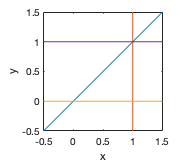
\includegraphics{img/C12-2dregion.png}

Construct the integral in the new order:
\begin{itemize}
\itemsep0em
    \item The inner integral is now with respect to $y$.  $y$ starts at $0$ for all values of $x$ and goes up to the line $x - y = 0$, so the line $y = x$.  
    \item The outer integral is with respect to $x$.  The `shadow' of the region on the $x$-axis is from $0$ to $1$.
    \item The function of integration (the integrand) does not change: $\displaystyle\int_0^1\int_0^x e^{x^2}\ dy\ dx$
\end{itemize}
\begin{align*}
    \int_0^1\int_0^x e^{x^2}\ dy\ dx &= \int_0^1\left[y e^{x^2}\right\vert_{y=0}^{y=x}\ dx \\
    &= \int_0^1 x e^{x^2}\ dx. \\
    \text{Let }u=x^2. & du = 2xdx\\
    \int_0^1\int_0^x e^{x^2}\ dy\ dx &= \int_{u=0^2}^{u=1^2} \frac{1}{2}e^u \ du \\
    &= \left[ \frac{1}{2}e^u\right\vert_0^1 \\
    &= \frac{1}{2}(e - 1).
\end{align*}


\vspace{0.2cm}
\hrule
\vspace{0.2cm}


% Example: wealth and income.  one is the integral of the other (approximately).  which way?

% mean temperature of the planet

% discounting requires an integral.

% any kind of weighting function will be a sum / integral

% averaging: take a running tally.  you're invoking the notion of an integral.  go back and forth between the discrete and continuous notions of an integral.

% food intake and weight gain.

% GDP.  GDP per capita vs for the country is a spatial average.  compare communities.  need a distribution function of GDP spatially and temporally.

% population: in the US the census is setting the discretization boxes for demographic data.



% Chain rule motivation: if there is a nonuniform pollutant field and a nonuniform temperature field, and I was moving.  What would I feel as a function of time?  I will experience it as a change in time but the change is a consequence of me moving through space.  There is a linear variation in temperature from the bottom of the grand canyon to the top.  Grab one of the temperature textbook problems.  Wrote a paper with Samuel... you think things are changing in time but its because you are moving.  Worms thermotax.
% grab an image from the paper.  fig 5cd. https://www.seas.harvard.edu/softmat/downloads/2006-12.pdf

% examples for triple integrals: 
% if an organism is moving through a liquid, and whatever is in the liquid is degrading and the organism samples over time, the organism sees an average value of the concentration (senses an average value).  Can they convert that word problem into an integral?  get rid of the path integral by sampling... $\phi$ is a function of time... average over all possible paths.  Blur the path integral and replace it with.


% can i look up some kind of simple volcanic island growth model.


\noindent\textbf{Teams}
You will work with this team on the in-class problems today.  ``Icebreaker'': share with your group something you have enjoyed reading.
\begin{multicols}{2}
1.  students here


\end{multicols}

%\vspace{0.2cm}
\hrule
\vspace{0.2cm}
\noindent\textbf{Setting up bounds for a double integral}

\noindent\textbf{Example (triangular region).}  Set up an iterated integral for $\int_R f\ dA$ where $f$ is an unknown function of two variables and $R$ is the triangular region shown below.

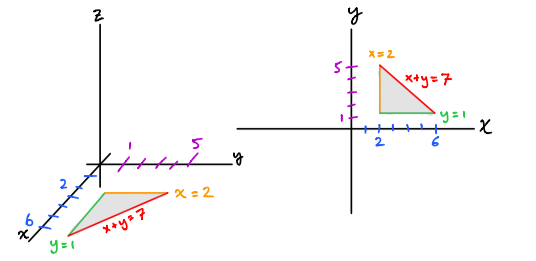
\includegraphics[width=3.5in]{img/C17p9-18.png}

\vfill

\noindent\textbf{Example (triangular region).}  For $R$ above, use iterated integrals to compute $\int_R (xy)\ dA$.

\vspace{1.5in}




\noindent\textbf{Example (half-disk region).}  Set up an iterated integral for $\int_R x\ dA$ where $f$ is as given in the integral, and $R$ is the half-disk shown below. %\emph{pollQ}

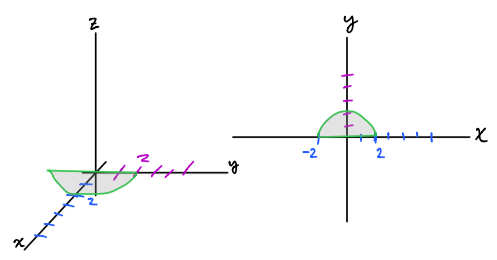
\includegraphics[width=3.5in]{img/C17p10-18.png}

\vspace{2in}


\noindent\textbf{Reading information from a double integral}

Let $I = \displaystyle\int_{-\sqrt{\pi}}^{\sqrt{\pi}}\int_0^{\sqrt{\pi-y^2}}\sin(x^2+y^2)dx dy$.
\begin{itemize}
    \item Identify the function of integration for $I$:
    \item Sketch the region of integration for the integral $I$.
    
  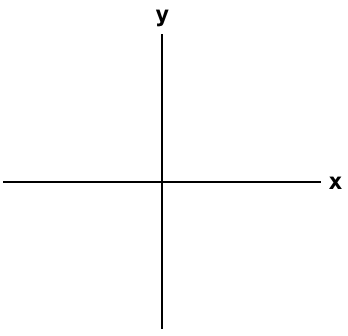
\includegraphics[height=2in]{img/C02axes-2.png}
\end{itemize}

\vspace{0.2cm}
\hrule
\vspace{0.2cm}

\eject

\noindent\textbf{Integration: triple integrals} \S 16.3
\begin{tcolorbox}
\begin{itemize}
\item The outer bounds will be constants.  The middle bounds may depend on the variable in the outer integral.  The inner bounds may depend on the middle and outer variables: $\displaystyle\int_{z=a}^{b}\int_{y=g_1(z)}^{g_2(z)}\int_{x=h_1(y,z)}^{h_2(y,z)}f(x,y,z)\ dx\ dy\ dz$
\item The innermost bounds convey much of the shape information.  \item To find the middle and outer bounds, find the `shadow' of the solid region on the coordinate plane associated with those variables ($xy$-plane of $xy$ are the outer two integrals, etc).  Construct the bounds for that shadow region in just the way you would construct bounds for a double integral. 
\end{itemize}
\end{tcolorbox}

\noindent\textbf{Example: setting up a triple integral to represent a solid region}. Consider the tetrahedron bounded by in the first octant and below the plane $3x + y + z = 1$. Let the density of this tetrahedron be $az$ g/cm$^3$ with position values $x,y,z$ measured in cm.  Set up an integral to find $M$, the mass of the tetrahedron.

%\emph{Set it up twice.  Once with $z$ as the inner integral, and once with $y$ as the inner integral.}

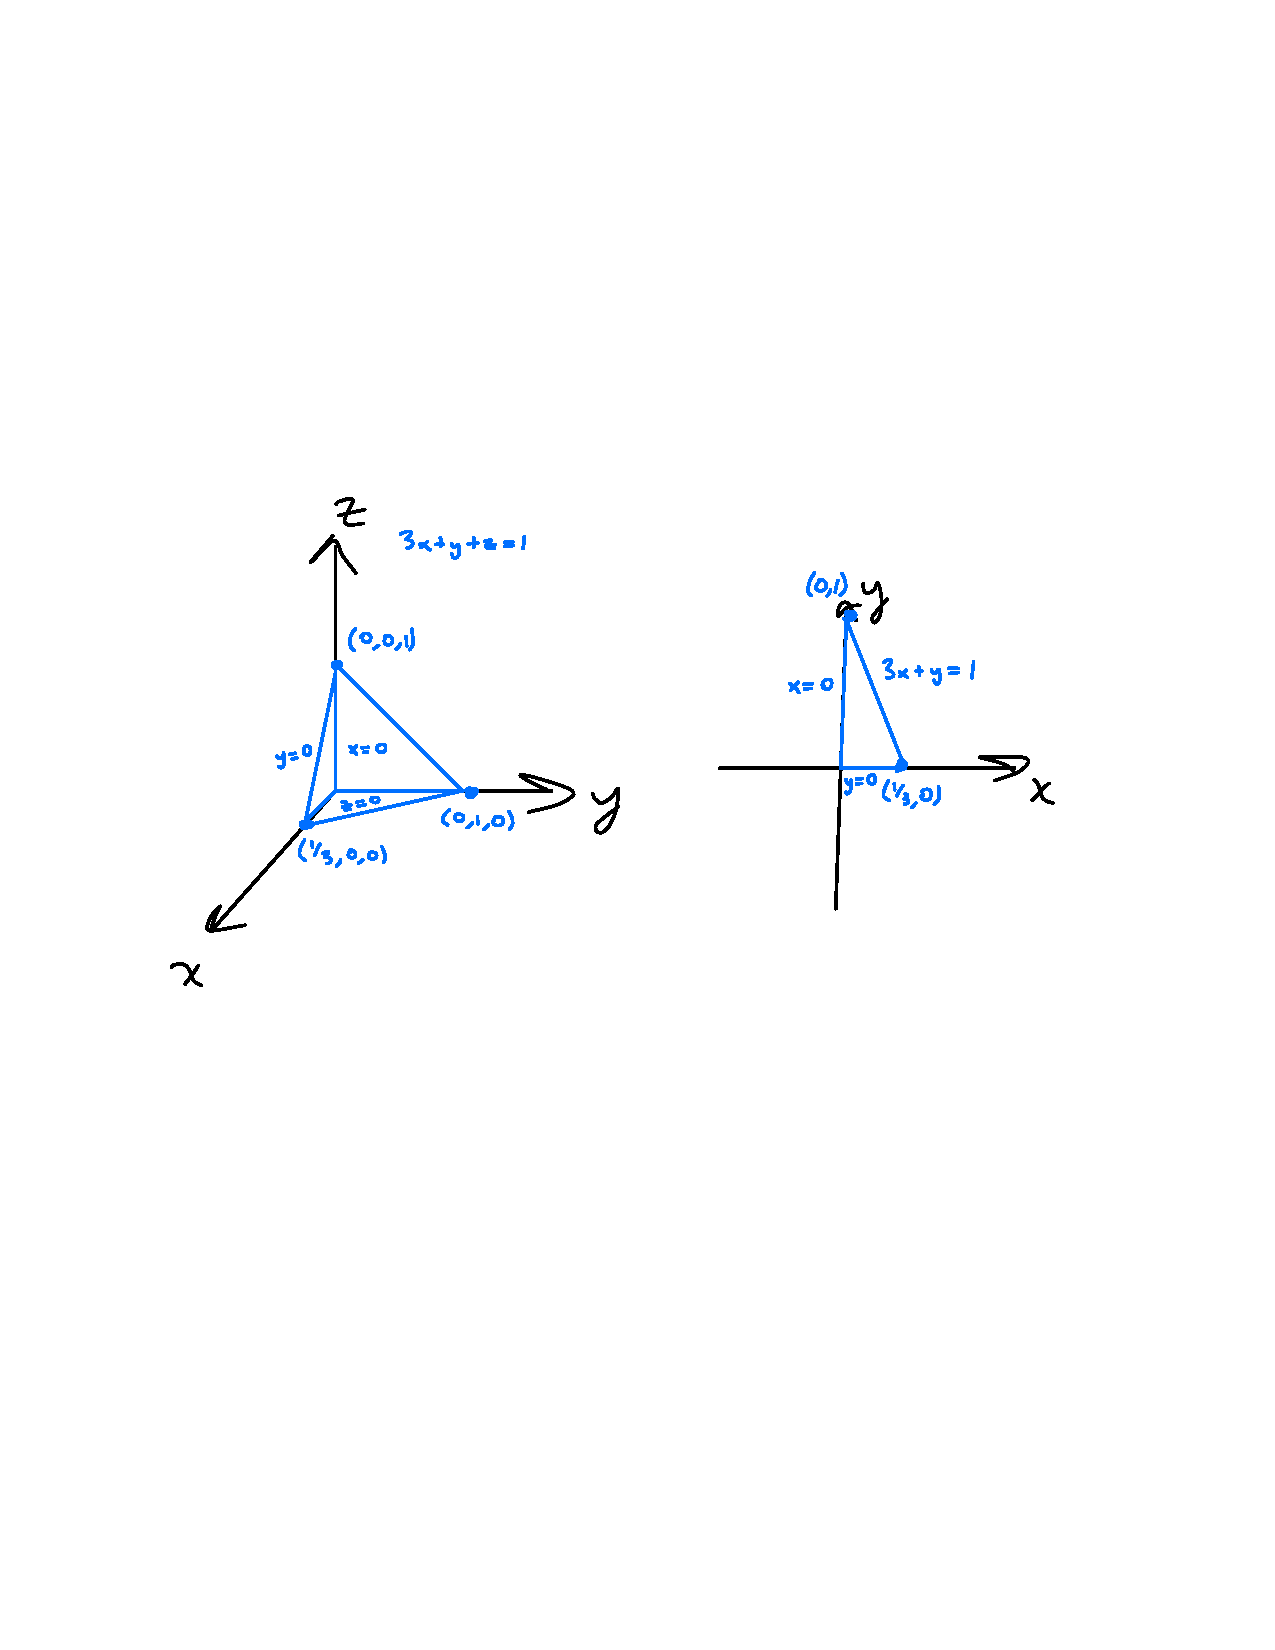
\includegraphics{img/N18_tetra.pdf}

\vfill


\noindent\textbf{Example (tetrahedron)}. For the tetrahedron above, set up an expression to find the mean density.
\vfill




\eject

\noindent\textbf{Example (region of integration).}  Change the order of integration for \[\int_0^1\int_{-1}^1\int_0^{\sqrt{1-z^2}}z\ dy\ dz\ dx\] to $\displaystyle\int_W f(x,y,z)\ dz\ dx\ dy$. 

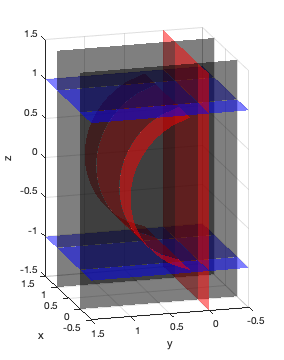
\includegraphics[height=2in]{img/C12-3dregion.png}

\begin{lstlisting}
syms x y z
fimplicit3(@(x,y,z) y,'facecolor','r','facealpha',0.5,'edgecolor','none')
hold on
fimplicit3(@(x,y,z) y-sqrt(1-z.^2),'facecolor','r','facealpha',0.5,'edgecolor','none')
fimplicit3(@(x,y,z) z+1,'facecolor','b','facealpha',0.5,'edgecolor','none')
fimplicit3(@(x,y,z) z-1,'facecolor','b','facealpha',0.5,'edgecolor','none')
fimplicit3(@(x,y,z) x,'facecolor','k','facealpha',0.5,'edgecolor','none')
fimplicit3(@(x,y,z) x-1,'facecolor','k','facealpha',0.5,'edgecolor','none')
axis([-0.5 1.5 -0.5 1.5 -1.5 1.5])
axis equal
xlabel('x'); ylabel('y'); zlabel('z')
\end{lstlisting}

\eject
\vspace{0.2cm}
\hrule
\vspace{0.2cm}

\noindent\textbf{Polar coordinates} \S 16.4

\begin{tcolorbox}

\begin{itemize}
\itemsep0em
    \item In polar coordinates, $x = r\cos\theta, y = r\sin\theta$.  $x^2+y^2 = r$.  
    \item The approximate area of a polar gridbox, $\Delta A$, is $\Delta A = (r\Delta\theta)\Delta r$, where $r\Delta\theta$ is the length of the circular arc and $\Delta r$ is the length of the radial segment.
    \item $\int_R f(x,y)\ dx\ dy = \int_R f(r\cos\theta,r\sin\theta)\ r\ dr\ d\theta$.
    \end{itemize}
    \end{tcolorbox}
    \begin{tcolorbox}

\begin{itemize}
\itemsep0em
    
    \item The conversion between $dxdy$ and $rdrd\theta$ can be found via the derivative (Jacobian) for the change of coordinates: Let $\underline x = \left(\begin{array}{c} x \\ y \end{array}\right)$ and $\underline u = \left(\begin{array}{c} r \\ \theta \end{array}\right)$.  We have $\dfrac{\partial \underline x}{\partial \underline u} = \left(\begin{array}{c c} \cos\theta & -r\sin\theta \\ \sin\theta & r\cos\theta \end{array}\right)$.  
    \item It turns out that $dA = 
    \left\vert\dfrac{\partial \underline x}{\partial \underline u}\right\vert d\overline{A}$ where $dA = dxdy$ and $d\overline{A} = drd\theta$.  $\dfrac{\partial \underline x}{\partial \underline u}$ is a linear transformation, and under the action of this transformation, a small box in $r,\theta$-space of area $d\overline{A}$ is transformed to a small box in $x,y$-space of area $dA = \left\vert\dfrac{\partial \underline x}{\partial \underline u}\right\vert d\overline{A}$.
\end{itemize}
\end{tcolorbox}


\noindent\textbf{Example (insect population).}  
The approximate population density of insects around a lake is estimated (in millions of insects per square kilometer) as shown in the figure below.  
\begin{itemize}
\itemsep0em
    \item The lake has a 2 km radius, and the outer circle has a 4 km radius.
\item Approximate the boxes as rectangles.  
\item The length of an arc of a circle is given by $r\Delta\theta$ where $r$ is the radius and $\Delta\Theta$ is the subtended angle.
\item Use a Riemann sum to estimate the total insect population that is within 1 km of the lake. 
\end{itemize}

 




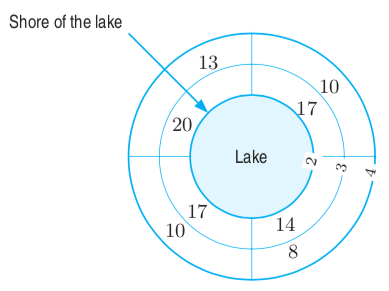
\includegraphics[width=2.5in]{img/C19p2.png}



\vspace{1in}

\noindent\textbf{Example: converting to polar}

Let $I = \displaystyle\int_{-\sqrt{\pi}}^{\sqrt{\pi}}\int_0^{\sqrt{\pi-y^2}}\sin(x^2+y^2)dx dy$.

To convert an integral from Cartesian to polar there are three steps:
\begin{enumerate}
    \item Convert the integrand: $\sin(x^2+y^2) = \sin(r^2)$.
    \item Convert $dA$:  $dxdy = rdrd\theta$.
    \item Convert the bounds:  Do this by converting the equations and sketching the region of integration.
    
    \begin{tabular}{| c c |}
        \hline
    $x = 0$ & $r\cos\theta = 0$ so $r = 0$ (not the case) or $\cos\theta = 0$, so $\theta = \pi/2$ or $\theta = -\pi/2$.\\
    \hline
    $x = \sqrt{\pi-y^2}$ & $\left\{\begin{array}{c} x^2+y^2 = \pi \\ x>0 \end{array}\right.$ so $\left\{\begin{array}{c}r^2 = \pi \\ -\pi/2<\theta<\pi/2\end{array}\right.$.  Simplifying,  $\left\{\begin{array}{c}r = \sqrt{\pi} \\ -\pi/2<\theta<\pi/2\end{array}\right.$\\
        \hline
    $y = -\sqrt{\pi}$ & $r\sin\theta = -\sqrt{\pi}$ \\
        \hline
    $y = \sqrt{\pi}$ & $r\sin\theta = \sqrt{\pi}$ \\
        \hline
    \end{tabular}
\end{enumerate}

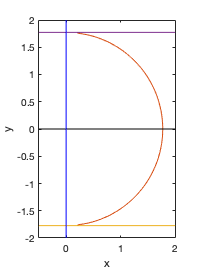
\includegraphics[height=2in]{img/C12-2dpolar.png}

 


\end{document}